\newpage
\section{Sơ đồ mạng và mô tả mã nguồn}
\subsection{Tổng quan}

\paragraph{Sơ đồ mạng:}{Các thành phần mạng trong đồ án được minh họa như hình bên dưới.}

\begin{figure}[H]
    \centering
    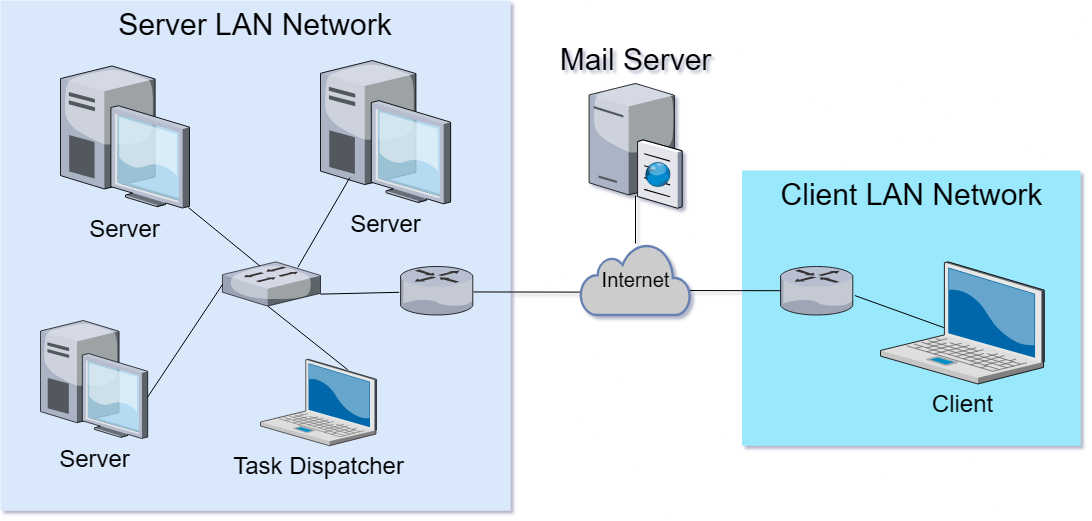
\includegraphics[width=1\linewidth]{img/net.png}
    \caption{Sơ đồ kết nối Client-Server thông qua mail}
\end{figure}

\paragraph{Cách hoạt động:}{Máy Client gửi lệnh và nghe phản hồi thông qua mail. Ở Server LAN Network, có một Task Dispatcher điều phối lệnh nhận được tới các máy Server để thực hiện nhiệm vụ.}

\paragraph{Phương pháp lập trình:}{Đồ án được lập trình theo phương pháp lập trình hướng thủ tục.}

\paragraph{Tổ chức mã nguồn:}{Mã nguồn (code) được tổ chức thành 2 thư mục chính: Client và Server, bao gồm các file với đuôi $.cpp$, $.h$, $.dll$, ... và các file thư viện khác. Trong đó, Client và Server chia sẻ chung một cách kết nối - gửi và nhận mail thông qua các hàm trong \texttt{mail.h}. Tuy nhiên, tùy theo Client và Server, sẽ có một phiên bản \texttt{mail.h} với sự bổ sung, chỉnh sửa phù hợp. }
\begin{itemize}
    \item \texttt{mail.h}: Định nghĩa các hàm dùng cURL, với phương thức IMAP và SMTP để gửi, nhận mail.
    \item \textbf{Server}: Thiết lập các Server và một Task Dispatcher (máy điều phối nhiệm vụ cho các Server).
    \begin{itemize}
        \item Gồm: \texttt{dispatcher.cpp}, \texttt{server.cpp}, \texttt{take\_screenshot.cpp}, \texttt{process.h}, \texttt{mail.h}.
    \end{itemize}
    
    \item \textbf{Client}: Thiết lập Client, gửi yêu cầu cho Server và nhận phản hồi. Cung cấp giao diện cho người dùng tương tác.
    \begin{itemize}
        \item Gồm: \texttt{client.cpp}, \texttt{mail.h}, các file $.dll$ (thư viện SDL), ảnh...
    \end{itemize}

    \item \textbf{Add-on}: File cài đặt OpenSSL và các file cần thiết khác.
\end{itemize}


\subsection{Chi tiết các thành phần code}

\subsubsection{Gửi/nhận mail - kết nối client-server}

\paragraph{File \texttt{mail.h}:}{\textbf{Định nghĩa các hàm sử dụng cURL để gửi, nhận email bằng giao thức SMTP, IMAP.}}

\paragraph{}{\textbf{Các hàm chính:}}

\begin{itemize}
    \item \texttt{sendMail} \texttt{(from, to, subject, body, userPass, fileName)}: Viết nội dung mail, gọi lệnh từ thư viện cURL để gửi mail bằng SMTP.
    \begin{itemize}
        \item \texttt{from}: Địa chỉ mail gửi.
        \item \texttt{to}: Địa chỉ mail nhận.
        \item \texttt{subject}: Tiêu đề mail.
        \item \texttt{body}: Nội dung mail.
        \item \texttt{userPass}: Mail và mật khẩu (app password\footnote{App Password: Mật khẩu ứng dụng được tạo riêng cho các ứng dụng của bên thứ ba truy cập tài khoản Google.}), dùng để xác thực thông tin gửi mail.
        \item \texttt{fileName}: Tên file đính kèm mail.
    \end{itemize}
        
    \item \texttt{newMail(client, task, numTask, fileContent)}: Thiết lập thông tin cần gửi (nơi gửi, loại yêu cầu, tên file đính kèm, mật khẩu...). Gọi hàm \texttt{sendMail} để gửi yêu cầu/phản hồi.
    \begin{itemize}
        \item \texttt{client}: Biến bool xác định Client hay Server gửi yêu cầu.
        \item \texttt{task}: Loại tác vụ yêu cầu/phản hồi.
        \item \texttt{numTask}: ID của tác vụ.
        \item \texttt{fileContent}: Tệp đính kèm (nếu có).
    \end{itemize}
        
    \item \texttt{readLatestMail(timeLISTEN, isClientLISTEN, MAIL, TASK)}: Đọc thông tin của mail mới nhất.
    \begin{itemize}
        \item \texttt{timeLISTEN}: Thời gian bắt đầu chạy Client/Server.
        \item \texttt{isClientLISTEN}: Biến bool xác định Client hay Server đang chạy.
        \item \texttt{MAIL}: Danh sách tiêu đề mail.
        \item \texttt{TASK}: Danh sách ID mail.
    \end{itemize}
        
    \item \texttt{autoGetMail(isClientLISTEN)}: Thiết lập một tiến trình liên tục lắng nghe tới mail server để nhận được mail mới nhất.
        \begin{itemize}
            \item \texttt{isClientLISTEN}: Biến bool xác định Client hay Server đang chạy.
        \end{itemize}
        
\end{itemize}
    
\paragraph{}{\textbf{Các hàm phụ:}}

\begin{itemize}
    \item \texttt{getCurrentDateTime()}: Lấy thông tin thời gian hiện tại.
        
    \item \texttt{base64\_encode(in)}: Mã hóa thông tin thành base64.
    \begin{itemize}
        \item \texttt{in}: Chuỗi kí tự base64 cần được giải mã.
    \end{itemize}
        
    \item \texttt{compareTimeStrings(timeStr1, timeStr2)}: So sánh 2 thời gian dạng chuỗi ký tự, để biết thời gian nào sớm/muộn hơn.
    \begin{itemize}
        \item \texttt{timeStr1}, \texttt{timeStr2}: 2 thời gian cần so sánh
    \end{itemize}
        
    \item \texttt{getID(userPass, isClientLISTEN)}: Dùng cURL và thông qua phương thức IMAP, gửi lệnh tới mail server yêu cầu nhận danh sách các mail có sẵn trong hộp thư.
    \begin{itemize}
        \item \texttt{userPass}: Địa chỉ mail và mật khẩu
        \item \texttt{isClientLISTEN}: Biến bool xác định là Client hay Server đang gửi yêu cầu
    \end{itemize}
        
    \item \texttt{readIDMail(orderNow)}: Đọc ID của mail mới nhất có trong hộp thư.
    \begin{itemize}
        \item \texttt{orderNow}: ID của mail hiện tại được trả về.
    \end{itemize}
        
    \item \texttt{getNewestMail(orderNow, userPass)}: Dùng cURL và thông qua phương thức IMAP, gửi lệnh tới mail server yêu cầu tải xuống mail mới nhất dựa trên ID đã lấy.
    \begin{itemize}
        \item \texttt{orderNow}: ID của mail hiện tại.
        \item \texttt{userPass}: Địa chỉ mail và mật khẩu
    \end{itemize}
        
    \item \texttt{extractInfo(subject, responseType, numTask, time)}: Trích xuất các yêu cầu trong mail đã tải. Xác nhận tính hợp lệ của mail.
    \begin{itemize}
        \item \texttt{subject}: Tiêu đề mail.
        \item \texttt{responseType}: Thể loại mail (request/response).
        \item \texttt{numTask}: ID của tác vụ.
        \item \texttt{time}: Thời gian gửi mail.
    \end{itemize}
        
        
    \item \texttt{base64\_decode(in)}: Giải mã thông tin base64.
    \begin{itemize}
        \item \texttt{in}: Chuỗi ký tự base64 cần được giải mã.
    \end{itemize}
        
    \item \texttt{saveFile(filename, data)}: Lưu tệp đính kèm mail (nếu có).
    \begin{itemize}
        \item \texttt{filename}: Tên file cần lưu.
        \item \texttt{data}: Dữ liệu của file đã được giải mã.
    \end{itemize}
    
\end{itemize}

\paragraph{}{File \texttt{mail.h} mẫu chỉ cung cấp các mẫu hàm để Server và Client có thể gửi, nhận lệnh thông qua mail. File \texttt{mail.h} riêng ở Server và Client có thể được chỉnh sửa cho phù hợp.}

\subsubsection{Server}

\paragraph{File \texttt{dispatcher.cpp}:}{\textbf{Khởi tạo tiến trình điều phối hoạt động các máy Server trong mạng LAN.}}
\begin{itemize}
    \item \texttt{sendTask(serverIP, numTask, request)}: Điều phối công việc đến server đang được điều khiển.
    \begin{itemize}
        \item \texttt{serverIP}: IP của server được điều khiển.
        \item \texttt{numTask}: Mã số của yêu cầu.
        \item \texttt{request}: Nội dung của yêu cầu.
    \end{itemize}

    \item \texttt{isPortOpen(ip, port)}: Kiểm tra xem một địa chỉ IP nào đó có đang mở cổng kết nối trên một Port nào đó hay không.
    \begin{itemize}
        \item \texttt{ip}: IP cần kiểm tra.
        \item \texttt{port}: Port cần kiểm tra.
    \end{itemize}

    \item \texttt{checkIP(serversIP, ip, port)}: kiểm tra một địa chỉ IP có phải một máy chủ đang lắng nghe hay không, nếu có thì bỏ vào \texttt{serversIP}.
    \begin{itemize}
        \item \texttt{serversIP}: Danh sách IP của các máy chủ.
        \item \texttt{ip}: IP cần kiểm tra.
        \item \texttt{port}: Port cần kiểm tra.
    \end{itemize}

    \item \texttt{getServersList(serversIP)}: Lấy danh sách IP của các server bỏ vào \texttt{serversIP}.
    \begin{itemize}
        \item \texttt{serversIP}: Danh sách IP của các máy chủ.
    \end{itemize}

    \item \texttt{handleRequest(serversIP, currentIP, numTask, request)}: Xử lý yêu cầu.
    \begin{itemize}
        \item \texttt{serversIP}: Danh sách IP của các máy chủ.
        \item \texttt{currentIP}: IP của server đang được điều khiển.
        \item \texttt{numTask}: Mã số của yêu cầu.
        \item \texttt{request}: Nội dung của yêu cầu.
    \end{itemize}

    \item \texttt{autoGetMail(serversIP)}: Lấy và đọc mail, thực hiện lắng nghe yêu cầu từ người dùng.
    \begin{itemize}
        \item \texttt{serversIP}: Danh sách IP của các máy chủ.
    \end{itemize}
\end{itemize}


\paragraph{File \texttt{server.cpp}:}{\textbf{Khởi tạo tiến trình trên một máy Server}.}
\begin{itemize}
    \item \texttt{start\_server()}: Khởi động chương trình và lưu lại đường dẫn của các ứng dụng.

    \item \texttt{createSocket()}: Thiết lập kết nối giao tiếp với chương trình điều phối

    \item \texttt{serveForever()}: Làm cho máy chủ hoạt động vô thời hạn.

    \item \texttt{handleRequest(numTask, request, socket)}: Xử lý các yêu cầu.
    \begin{itemize}
        \item \texttt{numTask}: Mã số của yêu cầu.
        \item \texttt{request}: Nội dung của yêu cầu.
        \item \texttt{socket}: Một socket giữa máy chủ và máy điều phối, sử dụng để đóng socket khi cần thiết.
    \end{itemize}

\end{itemize}

\paragraph{File \texttt{take\_screenshot.cpp}:}{\textbf{Chụp màn hình máy tính}.}
\begin{itemize}
    \item \texttt{takeScreenshot(Height, Width, targetHeight, targetWidth)}: chụp màn hình và lưu thành “screen.png”.
    \begin{itemize}
        \item \texttt{Height}: Chiều cao của màn hình.
        \item \texttt{Width}: Chiều rộng của màn hình.
        \item \texttt{targetHeight}: Chiều cao của ảnh đầu ra.
        \item \texttt{targetWidth}: Chiều rộng của ảnh đầu ra.
    \end{itemize}

\end{itemize}

\paragraph{File \texttt{process.h}:}{\textbf{Thực hiện các chức năng của Server}.}
\begin{itemize}
    \item \texttt{list\_apps()}: Tìm các file .exe và viết vào file “uploads/app\_list.txt” khi khởi động server.
        
    \item \texttt{list\_files(path)}: In ra các thư mục và file trong thư mục đường dẫn vào file “uploads/files\_list.txt”.
    \begin{itemize}
        \item \texttt{path}: Đường dẫn của thư mục cần liệt kê.
    \end{itemize}

    \item \texttt{run\_app(path)}: Chạy một chương trình .exe.
    \begin{itemize}
        \item \texttt{path}: Đường dẫn tuyệt đối của chương trình.exe.
    \end{itemize}

    \item \texttt{get\_screenshot()}: Thực thi chương trình phụ trợ “take\_screenshot.cpp” để chụp màn hình.

    \item \texttt{shut\_down()}: Ngưng hoạt động server và tắt nguồn server.

    \item \texttt{camera\_switch(cam\_status)}: Bật/tắt camera.
    \begin{itemize}
        \item \texttt{cam\_status}: 0/1 tương ứng với tắt hoặc bật camera.
    \end{itemize}

    \item \texttt{end\_task(task\_name)}: Ngừng một chương trình.
    \begin{itemize}
        \item \texttt{task\_name}: Tên chương trình dưới dạng <tên.exe>.
    \end{itemize}

    \item \texttt{bool end\_task\_PID(PID)}: Ngừng một chương trình theo PID.
    \begin{itemize}
        \item \texttt{PID}: PID của chương trình cần dừng.
    \end{itemize}

    \item \texttt{list\_running\_apps()}: Viết một danh sách các chương trình đang chạy vào file “uploads/running\_apps.txt”.
\end{itemize}
    
\newpage
\subsubsection{Client}

\paragraph{File \texttt{client.cpp}}{\textbf{Tạo tiến trình Client, cung cấp giao diện cho người dùng tương tác}.}

\paragraph{}{\textbf{Các hằng số, cấu trúc dữ liệu:}}
\begin{itemize}
    \item Kích thước và thông số màn hình:
    \begin{itemize}
        \item \texttt{SCREEN\_WIDTH = 800}: Xác định chiều rộng của cửa sổ app là 1786 pixel.
        \item \texttt{SCREEN\_HEIGHT = 600}: Xác định chiều cao của của sổ app là 868 pixel.
        % \item \texttt{MAX\_TEXT\_LENGTH = 20}: ?
        % \item \texttt{INITIAL\_SIDEBAR\_WIDTH = 50}: ?
        % \item \texttt{EXPANDED\_SIDEBAR\_WIDTH = 100}: ?
        % \item \texttt{TOGGLE\_BUTTON\_SIZE = 40}: ?
    \end{itemize}

    \item \texttt{enum Page}: Liệt kê các trang trong ứng dụng, bao gồm:
    \begin{itemize}
        \item \texttt{LOGIN}: Trang đăng nhập.
        \item \texttt{APP}: Trang chính của ứng dụng để giới thiệu đồ án và thành viên nhóm. 
        \item \texttt{REMOTE}: Trang điều kiển dành cho người dùng.
        \item \texttt{HELP}: Trang trợ giúp, thông tin.
    \end{itemize}

    \item \texttt{struct Sidebar}: Định nghĩa các thuộc tính của thanh bên.
    \begin{itemize}
        \item \texttt{currentPosition}: Vị trí hiện tại của thanh bên.
        \item \texttt{expanded}: Kiểm tra xem thanh bên có đang mở rộng hay không.
        \item \texttt{showBackButton}: Kiểm tra xem có hiển thị nút quay lại hay không.
    \end{itemize}

    % \item \texttt{struct ScrollBar}:
    % \begin{itemize}
    %     \item \texttt{yPosition}: ?
    %     \item \texttt{height}: ?
    %     \item \texttt{maxPosition}: ?
    % \end{itemize}
\end{itemize}


\paragraph{}{\textbf{Các hàm chính}:}
\begin{itemize}
    \item \texttt{runClient(stopClient)}: Khởi chạy giao diện người dùng.
    \begin{itemize}
        \item \texttt{stopClient}: Biến boolen, điều khiển việc dừng chương trình.
    \end{itemize}
    \item \texttt{runListen(stopClient)}: Khởi chạy tiến trình lắng nghe mail phản hồi.
    \begin{itemize}
        \item \texttt{stopClient}: Biến boolen, điều khiển việc dừng chương trình.
    \end{itemize}

    \item \texttt{toggleSidebar(sidebar)}: Thay đổi trạng thái của thanh bên (mở hoặc đóng).
    \begin{itemize}
        \item \texttt{sidebar}: Đối tượng thanh bên.
    \end{itemize}
    
    \item \texttt{renderText(renderer, font, text, x, y, color, maxWidth)}: Vẽ một đoạn văn bản lên màn hình. Sử dụng thư viện SDL để render văn bản bằng phông chữ TTF (TrueType Font).
    \begin{itemize}
        \item \texttt{renderer}: Đối tượng \texttt{SDL\_Renderer} dùng để vẽ lên màn hình.
        \item \texttt{font}: Đối tượng \texttt{TTF\_Font}, chứa thông tin về phông chữ được dùng để tạo văn bản.
        \item \texttt{text}: Chuỗi văn bản cần hiển thị.
        \item \texttt{x, y}: Tọa độ góc trên bên trái để bắt đầu vẽ văn bản.
        \item \texttt{color}: Màu sắc của văn bản, định nghĩa bằng đối tượng \texttt{SDL\_Color}.
        \item \texttt{maxWidth}: Chiều rộng tối đa mà văn bản có thể chiếm.
    \end{itemize}

    \item \texttt{renderSidebar(renderer, sidebar, font) }: Vẽ hình dạng và thông tin của thanh bên khi ở trong giao diện người dùng.
    \begin{itemize}
        \item \texttt{renderer}: Đối tượng \texttt{SDL\_Renderer} dùng để vẽ lên màn hình.
        \item \texttt{sidebar}: Đối tượng thanh bên.
        \item \texttt{font}: Đối tượng \texttt{TTF\_Font}, chứa thông tin về phông chữ được dùng để tạo văn bản.
    \end{itemize}
    
    \item \texttt{drawLoginPage(renderer, font, titleFont, username, password, registering, \\message, backgroundTexture)}: Vẽ trang đăng nhập hoặc đăng ký cho người dùng. Hiển thị các trường nhập liệu cho tên người dùng, mật khẩu và thông điệp (nếu có).
    \begin{itemize}
        \item \texttt{renderer}: Đối tượng \texttt{SDL\_Renderer} dùng để vẽ lên màn hình.
        \item \texttt{font, titleFont}: Phông chữ tiêu đề và văn bản thông thường.
        \item \texttt{username, password}: Thông tin tên người dùng và mật khẩu nhập vào.
        \item \texttt{registering}: Biến boolean cho biết người dùng có đang ở trang đăng ký hay không.
        \item \texttt{message}: Thông điệp hiển thị trên màn hình.
        \item \texttt{backgroundTexture}: Hình nền của trang.
    \end{itemize}

    \item \texttt{handleSidebarAction(itemIndex, running, loggedIn, renderer, font)}: Xử lý các \\hành động từ thanh bên (sidebar), ví dụ như đăng nhập, đăng xuất.
    \begin{itemize}
        \item \texttt{itemIndex}: Chỉ số mục được chọn trong thanh bên.
        \item \texttt{running}: Biến boolean cho biết ứng dụng còn đang chạy không.
        \item \texttt{loggedIn}: Biến boolean cho biết người dùng đã đăng nhập hay chưa.
        \item \texttt{renderer}: Đối tượng \texttt{SDL\_Renderer} dùng để vẽ lên màn hình.
        \item \texttt{font}: Phông chữ để render văn bản.
    \end{itemize}

    \item \texttt{drawAppPage(renderer, font, sidebar, backgroundTexture)}: Vẽ giao diện ứng dụng \\chính, bao gồm thanh bên và hình nền của trang.
    \begin{itemize}
        \item \texttt{renderer}: Đối tượng \texttt{SDL\_Renderer} dùng để vẽ lên màn hình.
        \item \texttt{font}: Đối tượng \texttt{TTF\_Font}, chứa thông tin về phông chữ được dùng để tạo văn bản.
        \item \texttt{sidebar}: Đối tượng \texttt{Sidebar} dùng để vẽ thanh bên của ứng dụng.
        \item \texttt{backgroundTexture}: Hình nền trang chính của ứng dụng.
    \end{itemize}

    \item \texttt{drawHelpPage(renderer, font, sidebar, backgroundTexture)}: Vẽ trang trợ giúp của \\ứng dụng.
    \begin{itemize}
        \item \texttt{renderer}: Đối tượng \texttt{SDL\_Renderer} dùng để vẽ lên màn hình.
        \item \texttt{font}: Phông chữ dùng để render văn bản trên trang trợ giúp.
        \item \texttt{sidebar}: Đối tượng \texttt{Sidebar} dùng để vẽ thanh bên trợ giúp.
        \item \texttt{backgroundTexture}: Hình nền của trang trợ giúp.
    \end{itemize}

    \item \texttt{drawSubmitButton(renderer, font)}: Vẽ nút "Send" trong trang Remote.
    \begin{itemize}
        \item \texttt{renderer}: Đối tượng \texttt{SDL\_Renderer} dùng để vẽ lên màn hình.
        \item \texttt{font}: Phông chữ dùng để render văn bản trên nút.
    \end{itemize}

    \item \texttt{drawButton(renderer, rect, text, font, color, textColor)}: Vẽ một nút với văn bản trên giao diện người dùng.
    \begin{itemize}
        \item \texttt{renderer}: Đối tượng \texttt{SDL\_Renderer} dùng để vẽ lên màn hình.
        \item \texttt{rect}: Đối tượng \texttt{SDL\_Rect} định nghĩa hình dạng và kích thước của nút.
        \item \texttt{text}: Văn bản hiển thị trên nút.
        \item \texttt{font}: Phông chữ dùng để render văn bản trên nút.
        \item \texttt{color}: Màu nền của nút.
        \item \texttt{textColor}: Màu của văn bản hiển thị trên nút.
    \end{itemize}

    \item \texttt{drawRemotePage(renderer, font, sidebar, option1Selected, option2Enabled, \\option2Title, processID, logMessages, option, selectedOptionText, \\backgroundTexture, imageTexture, loadImage, visibleLines, logHeight, \\scrollPosition)}: Vẽ trang điều khiển từ xa (remote), gồm các tùy chọn, thanh cuộn, log.
    \begin{itemize}
        \item \texttt{renderer}: Đối tượng \texttt{SDL\_Renderer}, dùng để vẽ lên màn hình.
        \item \texttt{font}: Đối tượng \texttt{TTF\_Font}, chứa thông tin về phông chữ được dùng để tạo văn bản.
        \item \texttt{sidebar}: Đối tượng \texttt{Sidebar} dùng để vẽ thanh bên.
        \item \texttt{option1Selected, option2Enabled}: Các biến boolean cho biết các tùy chọn có được chọn hoặc kích hoạt không.
        \item \texttt{option2Title}: Tiêu đề của tùy chọn 2.
        \item \texttt{processID}: ID của quá trình hiện tại.
        \item \texttt{logMessages}: Mảng chứa các thông điệp log hiển thị trên màn hình logConsole.
        \item \texttt{option}: Các tùy chọn hiện có cho người dùng.
        \item \texttt{selectedOptionText}:  Văn bản của tùy chọn đã chọn để gửi cho server.
        \item \texttt{backgroundTexture, imageTexture}: Hình nền và ảnh nền của trang.
        \item \texttt{loadImage}: Biến boolean cho biết có cần tải ảnh không.
        \item \texttt{visibleLines, logHeight}: Số dòng log hiển thị và chiều cao của phần log.
        \item \texttt{scrollPosition}: Vị trí hiện thị các câu lệnh trong trang Remote

    \end{itemize}
    
    \item \texttt{handleEvents(renderer, event, option1Selected, option, selectedOptionText,\\ loadImage, submitButton, processID, logMessages, tenfile, scrollPosition,\\ logHeight, visibleLines, imageTexture, check, font, sidebar, option2Enabled,\\ option2Title, backgroundTexture)}: Xử lý các sự kiện từ người dùng: nhấp chuột, cuộn chuột, cập nhật giao diện tương ứng của trang remote.
    \begin{itemize}
        \item \texttt{renderer}: Đối tượng \texttt{SDL\_Renderer}, dùng để vẽ lên màn hình.
        \item \texttt{event}: Đối tượng chứa thông tin sự kiện từ SDL (nhấp chuột, di chuyển chuột, ...).
        \item \texttt{option1Selected, option2Enabled, check}: Các biến boolean theo dõi trạng thái của các tùy chọn.
        \item \texttt{option}: Mảng các tùy chọn người dùng có thể chọn.
        \item \texttt{selectedOptionText}: Văn bản của tùy chọn hiện tại.
        \item \texttt{loadImage}: Biến boolean xác định có cần tải ảnh hay không.
        \item \texttt{submitButton}: Hình dạng của nút gửi.
        \item \texttt{processID}: ID của tiến trình.
        \item \texttt{logMessages}: Mảng chứa các thông điệp log.
        \item \texttt{tenfile}: Tên tệp hiện tại.
        \item \texttt{scrollPosition}: Vị trí của thanh cuộn.
        \item \texttt{logHeight, visibleLines}: Chiều cao của log và số dòng có thể hiển thị.
        \item \texttt{imageTexture}: Tải ảnh nếu cần thiết.
        \item \texttt{font}: Đối tượng \texttt{TTF\_Font}, chứa thông tin về phông chữ được dùng để tạo văn bản.
        \item \texttt{sidebar}: Thanh bên của ứng dụng.
        \item \texttt{option2Title}: Tiêu đề của tùy chọn thứ hai.
        \item \texttt{backgroundTexture}: Hình nền của trang.
    \end{itemize}

    \item \texttt{handleButtonClick(renderer, event, scrollPosition, visibleLines, totalLines,\\ upButton, downButton, clear, logMessages)}: Xử lý các hành động nhấp vào nút trên giao diện: cuộn lên, cuộn xuống, làm mới trong LogConsole.
    \begin{itemize}
        \item \texttt{renderer}: Đối tượng \texttt{SDL\_Renderer}, dùng để vẽ lên màn hình.
        \item \texttt{event}: Sự kiện nhấp chuột hoặc thao tác khác.
        \item \texttt{scrollPosition}: Vị trí của thanh cuộn.
        \item \texttt{visibleLines}: Số dòng log có thể hiển thị.
        \item \texttt{totalLines}: Tổng số dòng log.
        \item \texttt{upButton, downButton, clear}: Các nút trên giao diện để cuộn lên, cuộn xuống hoặc làm mới log.
        \item \texttt{logMessages}: Mảng chứa các thông điệp log.
    \end{itemize}

\end{itemize}

\paragraph{}{\textbf{Các hàm phụ:}}

\begin{itemize}
    \item \texttt{copyToClipboard(text)}: Sao chép văn bản vào bộ nhớ tạm (clipboard).
    \begin{itemize}
        \item \texttt{text}: Văn bản cần sao chép.
    \end{itemize}

    \item \texttt{pasteFromClipboard()}: Dán nội dung từ bộ nhớ tạm (clipboard).      

    \item \texttt{validateLogin(username, password)}: Kiểm tra tính hợp lệ của thông tin đăng nhập.
    \begin{itemize}
        \item \texttt{username, password}: Thông tin đăng nhập của người dùng.
    \end{itemize}

    \item \texttt{registerUser(username, password)}: Đăng ký người dùng mới.
    \begin{itemize}
        \item \texttt{username, password}: Thông tin đăng ký của người dùng mới.
    \end{itemize}
    
\end{itemize}